\section{Validation}

\subsection{1D Analytical Retardation Benchmark}

The first validation target is the tracked 1D case
\texttt{tutorials/reactiveTransport/reactiveScalarTransportDBSFoam/1DLinearRetardation}.
This case provides the dilute analytical benchmark used to verify the
field-level retardation factor and the expected reduction to retarded transport
in the linear-equilibrium limit.

The current benchmark compares:
\begin{itemize}
\item a surface-enabled moving case,
\item a matched aqueous-only moving case,
\item a dilute batch secant used to estimate $K_{s,\mathrm{field}}$.
\end{itemize}

For the current validated benchmark:
\begin{itemize}
\item $K_{s,\mathrm{field}} = 4.2412187733863601\times 10^{-6}$,
\item $R_{\mathrm{field}} = 2.6964875093545437$,
\item the mesh is $80 \times 1 \times 1$ with a species diffusion coefficient
of $10^{-11}\ \mathrm{m^2\,s^{-1}}$,
\item the surface-enabled profile matches the retarded advection-diffusion
reference with a relative L1 error of $0.75\%$ and a relative
$L_{\infty}$ error of $2.68\%$,
\item the aqueous-only profile matches its advection-diffusion reference with
a relative L1 error of $1.87\%$ and a relative $L_{\infty}$ error of
$8.44\%$,
\item the field-level total-equivalent inventory differs from the analytical
limit by $0.67\%$ for the surface-enabled run and $2.41\%$ for the
aqueous-only run.
\end{itemize}

These values are sufficient for the manuscript to claim that the production
solver reproduces the dilute field-level retardation limit of the current DBS
formulation. Figure 1 therefore focuses on the profile-level comparison rather
than a weak mean-only metric: the left panel shows the normalized aqueous
profile against the analytical advection-diffusion reference, and the right
panel shows the normalized adsorbed loading against the matching linear-limit
surface response.

\begin{figure}[htbp]
    \centering
    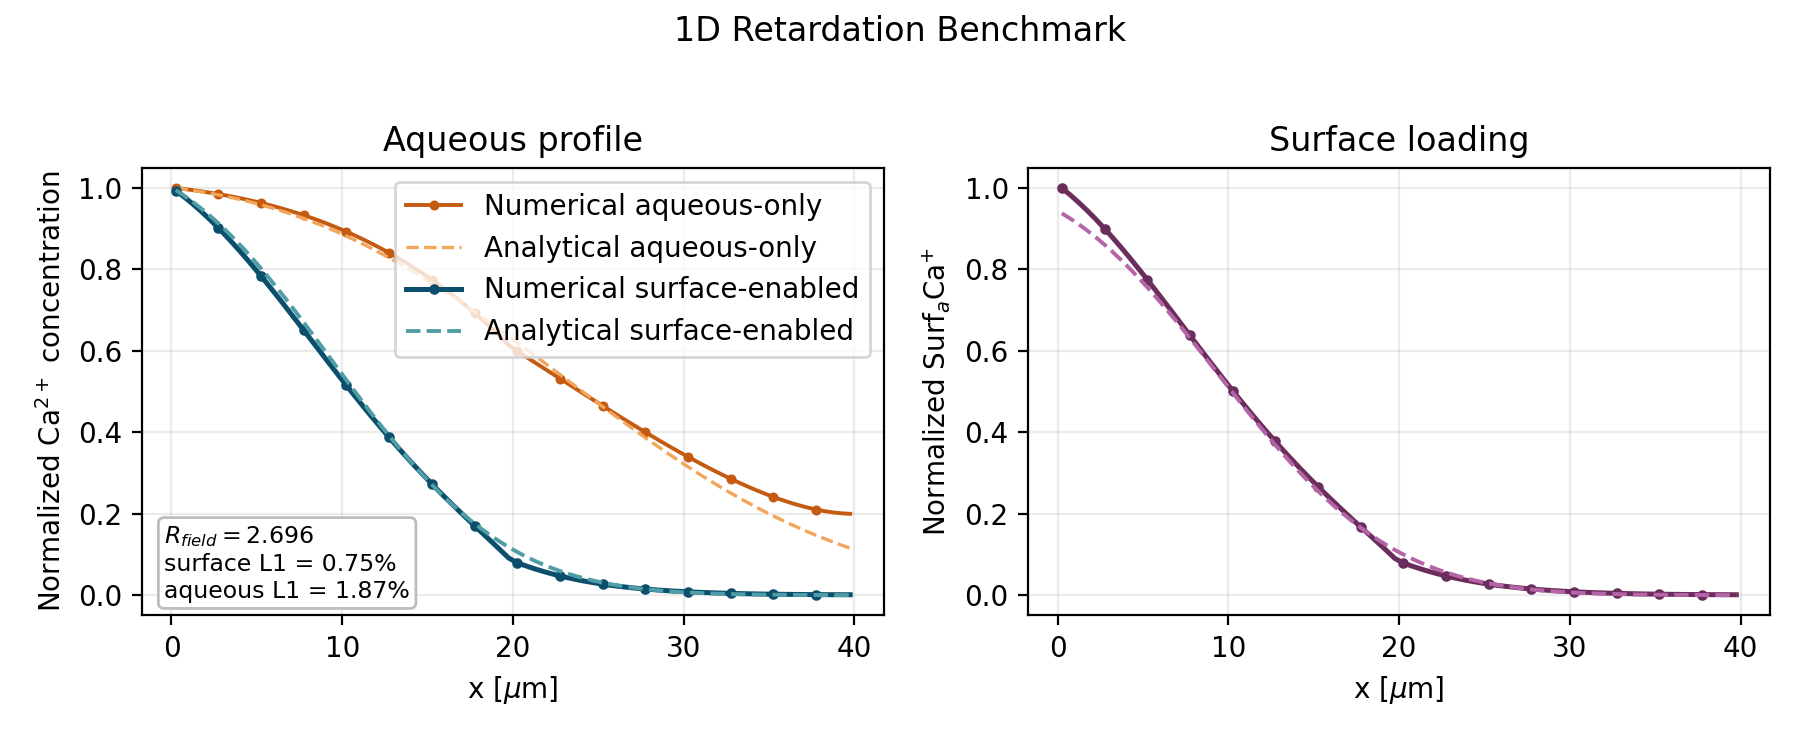
\includegraphics[width=0.9\linewidth]{figures/png/fig01_1d_retardation.png}
    \caption{1D analytical retardation benchmark. Left: normalized aqueous
    Ca$^{2+}$ profiles for the aqueous-only and surface-enabled runs, compared
    against their matching smooth advection-diffusion analytical solutions.
    Right: normalized surface loading compared against the linear-equilibrium
    analytical limit constructed from the calibrated field-level
    $K_{s,\mathrm{field}}$.}
\end{figure}

\subsection{Controlled Numerical Validation}

In addition to the analytical benchmark, the solver has been checked against a
set of controlled numerical baselines:
\begin{itemize}
\item aqueous-only reduction,
\item \mbox{$a_{\mathrm{surf}} = 0$} reduction,
\item closed-system adsorption and desorption,
\item decomposition, timestep, and mesh sensitivity on the fixed 1D benchmark.
\end{itemize}

These checks constrain both the mathematical correctness and the current
operating envelope used in the later image-based test cases.

\subsection{Validation Outputs Required For The Final Draft}

For the manuscript to be internally reviewable, the validation section should
end with a compact summary table containing:
\begin{itemize}
\item reduction-path pass/fail status,
\item analytical benchmark error,
\item decomposition sensitivity,
\item timestep sensitivity,
\item mesh sensitivity,
\item one representative chemistry-cost metric.
\end{itemize}

\begin{table}[htbp]
    \centering
    \caption{Placeholder for the validation summary table.}
    \begin{tabular}{lll}
        \toprule
        Check & Metric & Placeholder status \\
        \midrule
        Analytical 1D & Profile error / inventory drift & Drafted \\
        Decomposition & Total-equivalent drift & To be populated \\
        Timestep & Front-shape drift & To be populated \\
        Mesh & Front / total drift & To be populated \\
        Performance & Chemistry fraction & To be populated \\
        \bottomrule
    \end{tabular}
\end{table}
